\clearpage
\section{Результаты вычислительных экспериментов}
	Архитектуры, описанные в пункте 1.4.3, были реализованы в виде компьютерных программ на языке Python с помощью библиотеки для построения искусственных нейронных сетей Keras \cite{keras}, которая, в свою очередь, использует для расчетов пакет Tensorflow \cite{tf}. Использованные версии программных пакетов указаны в Приложении 1. Обучение проводилось на синтетических данных, сгенерированных самостоятельно реализованным генератором. 
	\subsection{Выборки с реализацией одного тренда}
		\subsubsection{Выборка 1}
			% sand:trend 2
			Выборка состояла из 3000 обучающих изображений и 500 валидационных. Частицами среды были круги диаметром 7 пикселей. Все изображения содержали в себе различные случайные реализации одного тренда интенсивности
			$$\lambda(x) = 0.2 + 0.01875x : \lambda_i = 0.2, \quad \lambda_f = 5$$
			
			Отличия в параметрах нейросетей указаны в (Таб. \ref{8-sand-trend2-nns}). Для всех обученных моделей параметр $\eta$, отвечающий за баланс между $L_{adv}$ и $L1$, был равен 100.
			
			\begin{table}[h!]
				\begin{center}
					\begin{tabular}{|c|c|c|}
						\hline
						Сеть & Число фильтров на первом слое & Сеть-генератор \\
						\hline
						nf8 & 8 & U-Net \\
						\hline
						nf16 & 16 & U-Net \\
						\hline
						nf16woU & 16 & Encoder-decoder \\
						\hline
						nf32 & 32 & U-Net \\
						\hline
					\end{tabular}
					\caption{Отличия в параметрах моделей (Выборка 1)}
					\label{8-sand-trend2-nns}
				\end{center}
			\end{table}
			
			Примеры синтеза, полученные с помощью нейросетей с различными параметрами, приведены в (Таб. \ref{8-dataset1-images}).
			
			\begin{table}[h!]
				\begin{center}
					\begin{tabular}{p{2cm} p{2cm} p{2cm} p{2cm} p{2cm} p{2cm} p{2cm}}
						\toprule
						Вход 1 & Вход 2 & Тренд & Сеть nf8 & nf16 & nf16woU & nf32 \\
						\cmidrule(r){1-1}\cmidrule(lr){2-2}\cmidrule(lr){3-3}\cmidrule(lr){4-4}\cmidrule(lr){5-5}\cmidrule(lr){6-6}\cmidrule(l){7-7}
						
\includegraphics[width=1\linewidth]{8-results/sand-trend2/left1}
						&
						
\includegraphics[width=1\linewidth]{8-results/sand-trend2/right1}
						&
						\includegraphics[width=1\linewidth]{8-results/sand-trend2/pan1}
						&
						
\includegraphics[width=1\linewidth]{8-results/sand-trend2/nf8/gen1}
						&
						
\includegraphics[width=1\linewidth]{8-results/sand-trend2/nf16/gen1}
						&
						
\includegraphics[width=1\linewidth]{8-results/sand-trend2/nf16_woUnet/gen1}
						&
						
\includegraphics[width=1\linewidth]{8-results/sand-trend2/nf32/gen1}
						\\
						\includegraphics[width=1\linewidth]{8-results/sand-trend2/left2}
						&
						\includegraphics[width=1\linewidth]{8-results/sand-trend2/right2}
						&
						\includegraphics[width=1\linewidth]{8-results/sand-trend2/pan2}
						&
						\includegraphics[width=1\linewidth]{8-results/sand-trend2/nf8/gen2}
						&
						\includegraphics[width=1\linewidth]{8-results/sand-trend2/nf16/gen2}
						&
						\includegraphics[width=1\linewidth]{8-results/sand-trend2/nf16_woUnet/gen2}
						&
						\includegraphics[width=1\linewidth]{8-results/sand-trend2/nf32/gen2}
						\\
						
\includegraphics[width=1\linewidth]{8-results/sand-trend2/left3}
						&
						
\includegraphics[width=1\linewidth]{8-results/sand-trend2/right3}
						&
						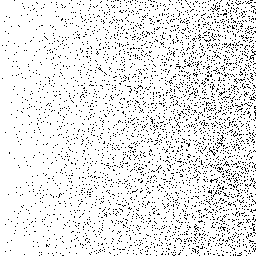
\includegraphics[width=1\linewidth]{8-results/sand-trend2/pan3}
						&
						\includegraphics[width=1\linewidth]{8-results/sand-trend2/nf8/gen3}
						&
						\includegraphics[width=1\linewidth]{8-results/sand-trend2/nf16/gen3}
						&
						\includegraphics[width=1\linewidth]{8-results/sand-trend2/nf16_woUnet/gen3}
						&
						\includegraphics[width=1\linewidth]{8-results/sand-trend2/nf32/gen3}
						\\
						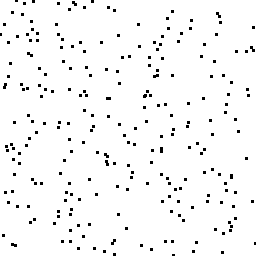
\includegraphics[width=1\linewidth]{8-results/sand-trend2/left4}
						&
						
\includegraphics[width=1\linewidth]{8-results/sand-trend2/right4}
						&
						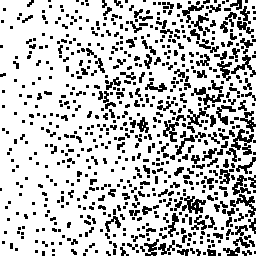
\includegraphics[width=1\linewidth]{8-results/sand-trend2/pan4}
						&
						\includegraphics[width=1\linewidth]{8-results/sand-trend2/nf8/gen4}
						&
						\includegraphics[width=1\linewidth]{8-results/sand-trend2/nf16/gen4}
						&
						\includegraphics[width=1\linewidth]{8-results/sand-trend2/nf16_woUnet/gen4}
						&
						\includegraphics[width=1\linewidth]{8-results/sand-trend2/nf32/gen4}
						\\
						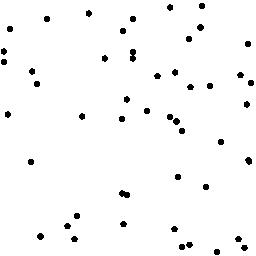
\includegraphics[width=1\linewidth]{8-results/sand-trend2/left5}
						&
						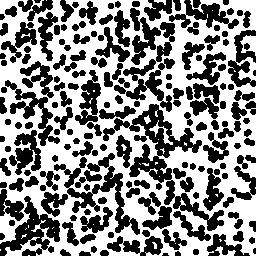
\includegraphics[width=1\linewidth]{8-results/sand-trend2/right5}
						&
						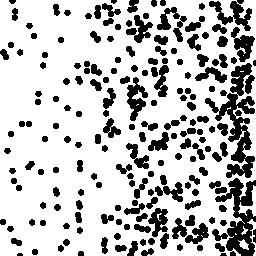
\includegraphics[width=1\linewidth]{8-results/sand-trend2/pan5}
						&
						
\includegraphics[width=1\linewidth]{8-results/sand-trend2/nf8/gen5}
						&
						
\includegraphics[width=1\linewidth]{8-results/sand-trend2/nf16/gen5}
						&
						
\includegraphics[width=1\linewidth]{8-results/sand-trend2/nf16_woUnet/gen5}
						&
						
\includegraphics[width=1\linewidth]{8-results/sand-trend2/nf32/gen5}
						\\
						\hline
					\end{tabular}
					\caption{Примеры синтеза (Выборка 1)}
					\label{8-dataset1-images}
				\end{center}
			\end{table}
			
			\break
			
			График приближения тренда различными сетями показан на (Рис. \ref{8-sand-trend2-results}).
			
			\begin{figure}[h!]
				\centering{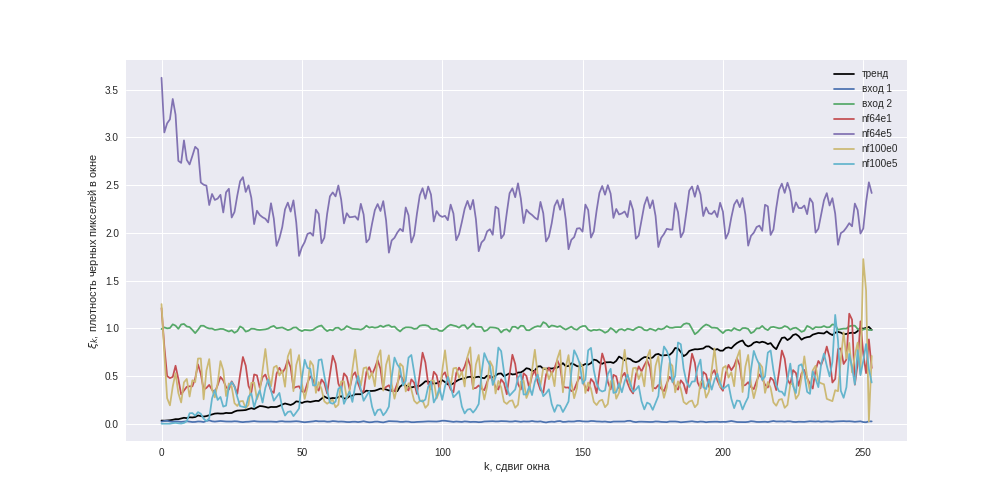
\includegraphics[width=\linewidth]{8-results/sand-trend2/results}}
				\caption{Аппроксимация тренда различными сетями (Выборка 1)}
				\label{8-sand-trend2-results}
			\end{figure}
			
			Значения введенной метрики для различных сетей указаны в (Таб. \ref{8-sand-trend2-metrics}).
			
			\begin{table}[h!]
				\begin{center}
					\begin{tabular}{|c|c|}
						\hline
						Сеть & Метрика \\
						\hline
						nf16woU & 0.24048\\
						\hline
						nf8 & 0.22511\\
						\hline
						nf16 & 0.18844\\
						\hline
						nf32 & 0.14589\\
						\hline
					\end{tabular}
					\caption{Значения метрики для разных сетей (меньше - лучше)}
					\label{8-sand-trend2-metrics}
				\end{center}
			\end{table}
			
			Лучшей по введенной метрике оказалась сеть nf32.
		\subsubsection{Выборка 2}
			% sand:trend 8
			Выборка состояла из 6000 обучающих изображений и 316 валидационных. Частицами среды были квадраты стороной 3 пикселя. Все изображения содержали в себе различные случайные реализации одного тренда интенсивности
			$$\lambda(x) = 1 + 0.0546875x: \lambda_i = 1, \quad \lambda_f = 15$$
			
			Отличия в параметрах обученных нейросетей указаны в (Таб. \ref{8-sand-trend8-nns}). Во всех обученных моделях в качестве сети-генератора использовалась сеть ``U-Net''.
			
			\begin{table}[h!]
				\begin{center}
					\begin{tabular}{|c|c|c|c|}
						\hline
						Сеть & Число фильтров на первом слое & $\eta$ & Метод оптимизации\\
						\hline
						nf32e5 & 32 & 5 & Adam \\
						\hline
						nf64e1 & 64 & 1 & RMSprop \\
						\hline
						nf64e5 & 64 & 5 & RMSprop \\
						\hline
						nf64e10 & 65 & 10 & RMSprop \\
						\hline
					\end{tabular}
					\caption{Отличия в параметрах моделей (Выборка 2)}
					\label{8-sand-trend8-nns}
				\end{center}
			\end{table}
			
			Примеры синтеза, полученные с помощью нейросетей с различными параметрами, приведены в (Таб. \ref{8-dataset2-images}).
			\begin{table}[h!]
				\begin{center}
					\begin{tabular}{p{2cm} p{2cm} p{2cm} p{2cm} p{2cm} p{2cm} p{2cm}}
						\toprule
						Вход 1 & Вход 2 & Тренд & Сеть nf32e5 & nf64e1 & nf64e5 & nf64e10 \\
						\cmidrule(r){1-1}\cmidrule(lr){2-2}\cmidrule(lr){3-3}\cmidrule(lr){4-4}\cmidrule(lr){5-5}\cmidrule(lr){6-6}\cmidrule(l){7-7}
						
\includegraphics[width=1\linewidth]{8-results/sand-trend8/left1}
						&
						
\includegraphics[width=1\linewidth]{8-results/sand-trend8/right1}
						&
						\includegraphics[width=1\linewidth]{8-results/sand-trend8/pan1}
						&
						
\includegraphics[width=1\linewidth]{8-results/sand-trend8/nf32e5/gen1}
						&
						
\includegraphics[width=1\linewidth]{8-results/sand-trend8/nf64e1/gen1}
						&
						
\includegraphics[width=1\linewidth]{8-results/sand-trend8/nf64e5/gen1}
						&
						
\includegraphics[width=1\linewidth]{8-results/sand-trend8/nf64e10/gen1}
						\\
						\includegraphics[width=1\linewidth]{8-results/sand-trend8/left2}
						&
						\includegraphics[width=1\linewidth]{8-results/sand-trend8/right2}
						&
						\includegraphics[width=1\linewidth]{8-results/sand-trend8/pan2}
						&
						\includegraphics[width=1\linewidth]{8-results/sand-trend8/nf32e5/gen2}
						&
						\includegraphics[width=1\linewidth]{8-results/sand-trend8/nf64e1/gen2}
						&
						\includegraphics[width=1\linewidth]{8-results/sand-trend8/nf64e5/gen2}
						&
						\includegraphics[width=1\linewidth]{8-results/sand-trend8/nf64e10/gen2}
						\\
						\includegraphics[width=1\linewidth]{8-results/sand-trend8/left3}
						&
						\includegraphics[width=1\linewidth]{8-results/sand-trend8/right3}
						&
						\includegraphics[width=1\linewidth]{8-results/sand-trend8/pan3}
						&
						\includegraphics[width=1\linewidth]{8-results/sand-trend8/nf32e5/gen3}
						&
						\includegraphics[width=1\linewidth]{8-results/sand-trend8/nf64e1/gen3}
						&
						\includegraphics[width=1\linewidth]{8-results/sand-trend8/nf64e5/gen3}
						&
						\includegraphics[width=1\linewidth]{8-results/sand-trend8/nf64e10/gen3}
						\\
						\includegraphics[width=1\linewidth]{8-results/sand-trend8/left4}
						&
						\includegraphics[width=1\linewidth]{8-results/sand-trend8/right4}
						&
						\includegraphics[width=1\linewidth]{8-results/sand-trend8/pan4}
						&
						\includegraphics[width=1\linewidth]{8-results/sand-trend8/nf32e5/gen4}
						&
						\includegraphics[width=1\linewidth]{8-results/sand-trend8/nf64e1/gen4}
						&
						\includegraphics[width=1\linewidth]{8-results/sand-trend8/nf64e5/gen4}
						&
						\includegraphics[width=1\linewidth]{8-results/sand-trend8/nf64e10/gen4}
						\\
						\includegraphics[width=1\linewidth]{8-results/sand-trend8/left5}
						&
						\includegraphics[width=1\linewidth]{8-results/sand-trend8/right5}
						&
						\includegraphics[width=1\linewidth]{8-results/sand-trend8/pan5}
						&
						\includegraphics[width=1\linewidth]{8-results/sand-trend8/nf32e5/gen5}
						&
						\includegraphics[width=1\linewidth]{8-results/sand-trend8/nf64e1/gen5}
						&
						\includegraphics[width=1\linewidth]{8-results/sand-trend8/nf64e5/gen5}
						&
						\includegraphics[width=1\linewidth]{8-results/sand-trend8/nf64e10/gen5}
						\\
						\hline
					\end{tabular}
					\caption{Примеры синтеза (Выборка 2)}
					\label{8-dataset2-images}
				\end{center}
			\end{table}
			
			\break
			
			График приближения тренда различными сетями показан на (Рис. \ref{8-sand-trend8-results}).
			
			\begin{figure}[h!]
				\centering{\includegraphics[width=\linewidth]{8-results/sand-trend8/results}}
				\caption{Аппроксимация тренда различными сетями (Выборка 2)}
				\label{8-sand-trend8-results}
			\end{figure}
			
			Значения введенной метрики для различных сетей указаны в (Таб. \ref{8-sand-trend8-metrics}).
			
			\begin{table}[h!]
				\begin{center}
					\begin{tabular}{|c|c|}
						\hline
						Сеть & Метрика \\
						\hline
						nf64e10 & 0.11168\\
						\hline
						nf64e5 & 0.06501\\
						\hline
						nf32e5 & 0.04827\\
						\hline
						nf64e1 & 0.01393\\
						\hline
					\end{tabular}
					\caption{Значения метрики для разных сетей (меньше - лучше)}
					\label{8-sand-trend8-metrics}
				\end{center}
			\end{table}
			
			Лучшей по введенной метрике оказалась сеть nf64e1.
		\subsubsection{Выборка 3}
			% dust:trend 1
			Выборка состояла из 6000 обучающих изображений и 316 валидационных. Частицами среды были единичные пиксели. Все изображения содержали в себе различные случайные реализации одного тренда интенсивности
			$$тут формула \lambda(x) = 1 + 0.19140625x: \lambda_i = 1, \quad \lambda_f = 50$$
			
			Отличия в параметрах обученных нейросетей указаны в (Таб. \ref{8-dust-trend1-nns}). Во всех обученных моделях в качестве сети-генератора использовалась сеть ``U-Net''. В качестве метода оптимизации использовался Adam.
			
			\begin{table}[h!]
				\begin{center}
					\begin{tabular}{|c|c|c|}
						\hline
						Сеть & Число фильтров на первом слое & $\eta$ \\
						\hline
						nf64e1 & 64 & 1 \\
						\hline
						nf64e5 & 64 & 5 \\
						\hline
						nf100e0 & 100 & 0 \\
						\hline
						nf100e5 & 100 & 5 \\
						\hline
					\end{tabular}
					\caption{Отличия в параметрах моделей (Выборка 3)}
					\label{8-dust-trend1-nns}
				\end{center}
			\end{table}
			
			Примеры синтеза, полученные с помощью нейросетей с различными параметрами, приведены в (Таб. \ref{8-dataset3-images}).
			\begin{table}[h!]
				\begin{center}
					\begin{tabular}{p{2cm} p{2cm} p{2cm} p{2cm} p{2cm} p{2cm} p{2cm}}
						\toprule
						Вход 1 & Вход 2 & Тренд & Сеть nf64e1 & nf64e5 & nf100e0 & nf100e5 \\
						\cmidrule(r){1-1}\cmidrule(lr){2-2}\cmidrule(lr){3-3}\cmidrule(lr){4-4}\cmidrule(lr){5-5}\cmidrule(lr){6-6}\cmidrule(l){7-7}
						\includegraphics[width=1\linewidth]{8-results/dust-trend1/left1}
						&
						\includegraphics[width=1\linewidth]{8-results/dust-trend1/right1}
						&
						\includegraphics[width=1\linewidth]{8-results/dust-trend1/pan1}
						&
						\includegraphics[width=1\linewidth]{8-results/dust-trend1/nf64e1/gen1}
						&
						\includegraphics[width=1\linewidth]{8-results/dust-trend1/nf64e5/gen1}
						&
						\includegraphics[width=1\linewidth]{8-results/dust-trend1/nf100e0/gen1}
						&
						\includegraphics[width=1\linewidth]{8-results/dust-trend1/nf100e5/gen1}
						\\
						\includegraphics[width=1\linewidth]{8-results/dust-trend1/left2}
						&
						\includegraphics[width=1\linewidth]{8-results/dust-trend1/right2}
						&
						\includegraphics[width=1\linewidth]{8-results/dust-trend1/pan2}
						&
						\includegraphics[width=1\linewidth]{8-results/dust-trend1/nf64e1/gen2}
						&
						\includegraphics[width=1\linewidth]{8-results/dust-trend1/nf64e5/gen2}
						&
						\includegraphics[width=1\linewidth]{8-results/dust-trend1/nf100e0/gen2}
						&
						\includegraphics[width=1\linewidth]{8-results/dust-trend1/nf100e5/gen2}
						\\
						\includegraphics[width=1\linewidth]{8-results/dust-trend1/left3}
						&
						\includegraphics[width=1\linewidth]{8-results/dust-trend1/right3}
						&
						\includegraphics[width=1\linewidth]{8-results/dust-trend1/pan3}
						&
						\includegraphics[width=1\linewidth]{8-results/dust-trend1/nf64e1/gen3}
						&
						\includegraphics[width=1\linewidth]{8-results/dust-trend1/nf64e5/gen3}
						&
						\includegraphics[width=1\linewidth]{8-results/dust-trend1/nf100e0/gen3}
						&
						\includegraphics[width=1\linewidth]{8-results/dust-trend1/nf100e5/gen3}
						\\
						\includegraphics[width=1\linewidth]{8-results/dust-trend1/left4}
						&
						\includegraphics[width=1\linewidth]{8-results/dust-trend1/right4}
						&
						\includegraphics[width=1\linewidth]{8-results/dust-trend1/pan4}
						&
						\includegraphics[width=1\linewidth]{8-results/dust-trend1/nf64e1/gen4}
						&
						\includegraphics[width=1\linewidth]{8-results/dust-trend1/nf64e5/gen4}
						&
						\includegraphics[width=1\linewidth]{8-results/dust-trend1/nf100e0/gen4}
						&
						\includegraphics[width=1\linewidth]{8-results/dust-trend1/nf100e5/gen4}
						\\
						\includegraphics[width=1\linewidth]{8-results/dust-trend1/left5}
						&
						\includegraphics[width=1\linewidth]{8-results/dust-trend1/right5}
						&
						\includegraphics[width=1\linewidth]{8-results/dust-trend1/pan5}
						&
						\includegraphics[width=1\linewidth]{8-results/dust-trend1/nf64e1/gen5}
						&
						\includegraphics[width=1\linewidth]{8-results/dust-trend1/nf64e5/gen5}
						&
						\includegraphics[width=1\linewidth]{8-results/dust-trend1/nf100e0/gen5}
						&
						\includegraphics[width=1\linewidth]{8-results/dust-trend1/nf100e5/gen5}
						\\
						\hline
					\end{tabular}
					\caption{Примеры синтеза (Выборка 3)}
					\label{8-dataset3-images}
				\end{center}
			\end{table}
			
			\break
			
			График приближения тренда различными сетями показан на (Рис. \ref{8-dust-trend1-results}).
			
			\begin{figure}[h!]
				\centering{\includegraphics[width=\linewidth]{8-results/dust-trend1/results}}
				\caption{Аппроксимация тренда различными сетями (Выборка 3)}
				\label{8-dust-trend1-results}
			\end{figure}
			
			Значения введенной метрики для различных сетей указаны в (Таб. \ref{8-dust-trend1-metrics}).
			
			\begin{table}[h!]
				\begin{center}
					\begin{tabular}{|c|c|}
						\hline
						Сеть & Метрика \\
						\hline
						nf64e5 & 3.13633\\
						\hline
						nf100e0 & 0.1178\\
						\hline
						nf100e5 & 0.08266\\
						\hline
						nf64e1 & 0.08139\\
						\hline
					\end{tabular}
					\caption{Значения метрики для разных сетей (меньше - лучше)}
					\label{8-dust-trend1-metrics}
				\end{center}
			\end{table}
			
			Лучшей по введенной метрике оказалась сеть nf64e1. Однако видно, что на этой выборке сети не смогли распознать тренд, и сошлись примерно к средней по выборке интенсивности (не учитывая сети nf64e5, явно являющейся выбросом).
		
	\subsection{Выборки с реализацией различных трендов}
		\subsubsection{Выборка 4}
			% dust: trend 2
			Выборка состояла из 6000 обучающих изображений и 316 валидационных. Частицами среды были единичные пиксели. Все изображения содержали в себе различные случайные реализации разных трендов интенсивности $\lambda(x)$
			$$ \lambda_{init}, \lambda_{final} \sim \mathcal{U}\{0, 50\}, $$
			то есть, значения $\lambda_{init}$ и $\lambda_{final}$ для каждого отдельного экземпляра выбирались случайно.
			
			Отличия в параметрах обученных нейросетей указаны в (Таб. \ref{8-dust-trend2-nns}). Во всех обученных моделях в качестве сети-генератора использовалась сеть ``U-Net''. Каждая сеть была обучена как с помощью Adam, так и с помощью RMSprop.
			
			\begin{table}[h!]
				\begin{center}
					\begin{tabular}{|c|c|c|}
						\hline
						Сеть & Число фильтров на первом слое & $\eta$ \\
						\hline
						nf32e5 & 32 & 5 \\
						\hline
						nf32e10 & 32 & 10 \\
						\hline
						nf32e20 & 32 & 20 \\
						\hline
						nf32e50 & 32 & 50 \\
						\hline
					\end{tabular}
					\caption{Отличия в параметрах моделей (Выборка 3)}
					\label{8-dust-trend2-nns}
				\end{center}
			\end{table}
			
			Примеры синтеза, полученные с помощью нейросетей с различными параметрами, приведены в (Таб. \ref{8-dataset4-images}).
			\begin{table}[h!]
				\begin{center}
					\begin{tabular}{p{2cm} p{2cm} p{2cm} p{2cm} p{2cm} p{2cm} p{2cm}}
						\toprule
						Вход 1 & Вход 2 & Тренд & Сеть nf32e5 & nf32e10 & nf32e20 & nf32e50 \\
						\cmidrule(r){1-1}\cmidrule(lr){2-2}\cmidrule(lr){3-3}\cmidrule(lr){4-4}\cmidrule(lr){5-5}\cmidrule(lr){6-6}\cmidrule(l){7-7}
						\includegraphics[width=1\linewidth]{8-results/dust-trend2/left1}
						&
						\includegraphics[width=1\linewidth]{8-results/dust-trend2/right1}
						&
						\includegraphics[width=1\linewidth]{8-results/dust-trend2/pan1}
						&
						\includegraphics[width=1\linewidth]{8-results/dust-trend2/nf32e5/gen1}
						&
						\includegraphics[width=1\linewidth]{8-results/dust-trend2/nf32e10/gen1}
						&
						\includegraphics[width=1\linewidth]{8-results/dust-trend2/nf32e20/gen1}
						&
						\includegraphics[width=1\linewidth]{8-results/dust-trend2/nf32e50/gen1}
						\\
						\includegraphics[width=1\linewidth]{8-results/dust-trend2/left2}
						&
						\includegraphics[width=1\linewidth]{8-results/dust-trend2/right2}
						&
						\includegraphics[width=1\linewidth]{8-results/dust-trend2/pan2}
						&
						\includegraphics[width=1\linewidth]{8-results/dust-trend2/nf32e5/gen2}
						&
						\includegraphics[width=1\linewidth]{8-results/dust-trend2/nf32e10/gen2}
						&
						\includegraphics[width=1\linewidth]{8-results/dust-trend2/nf32e20/gen2}
						&
						\includegraphics[width=1\linewidth]{8-results/dust-trend2/nf32e50/gen2}
						\\
						\includegraphics[width=1\linewidth]{8-results/dust-trend2/left3}
						&
						\includegraphics[width=1\linewidth]{8-results/dust-trend2/right3}
						&
						\includegraphics[width=1\linewidth]{8-results/dust-trend2/pan3}
						&
						\includegraphics[width=1\linewidth]{8-results/dust-trend2/nf32e5/gen3}
						&
						\includegraphics[width=1\linewidth]{8-results/dust-trend2/nf32e10/gen3}
						&
						\includegraphics[width=1\linewidth]{8-results/dust-trend2/nf32e20/gen3}
						&
						\includegraphics[width=1\linewidth]{8-results/dust-trend2/nf32e50/gen3}
						\\
						\includegraphics[width=1\linewidth]{8-results/dust-trend2/left4}
						&
						\includegraphics[width=1\linewidth]{8-results/dust-trend2/right4}
						&
						\includegraphics[width=1\linewidth]{8-results/dust-trend2/pan4}
						&
						\includegraphics[width=1\linewidth]{8-results/dust-trend2/nf32e5/gen4}
						&
						\includegraphics[width=1\linewidth]{8-results/dust-trend2/nf32e10/gen4}
						&
						\includegraphics[width=1\linewidth]{8-results/dust-trend2/nf32e20/gen4}
						&
						\includegraphics[width=1\linewidth]{8-results/dust-trend2/nf32e50/gen4}
						\\
						\includegraphics[width=1\linewidth]{8-results/dust-trend2/left5}
						&
						\includegraphics[width=1\linewidth]{8-results/dust-trend2/right5}
						&
						\includegraphics[width=1\linewidth]{8-results/dust-trend2/pan5}
						&
						\includegraphics[width=1\linewidth]{8-results/dust-trend2/nf32e5/gen5}
						&
						\includegraphics[width=1\linewidth]{8-results/dust-trend2/nf32e10/gen5}
						&
						\includegraphics[width=1\linewidth]{8-results/dust-trend2/nf32e20/gen5}
						&
						\includegraphics[width=1\linewidth]{8-results/dust-trend2/nf32e50/gen5}
						\\
						\hline
					\end{tabular}
					\caption{Примеры синтеза (Выборка 4)}
					\label{8-dataset4-images}
				\end{center}
			\end{table}
			
			График приближения тренда различными сетями показан на (Рис. \ref{8-dust-trend2-results}).
			
			\begin{figure}[h!]
				\centering{\includegraphics[width=\linewidth]{8-results/dust-trend2/results}}
				\caption{Аппроксимация тренда различными сетями (Выборка 4)}
				\label{8-dust-trend2-results}
			\end{figure}
			
			Значения введенной метрики для различных сетей указаны в (Таб. \ref{8-dust-trend2-metrics}).
			
			\begin{table}[h!]
				\begin{center}
					\begin{tabular}{|c|c|}
						\hline
						Сеть & Метрика \\
						\hline
						nf32e5 & 1.27751\\
						\hline
						nf32e50 & 0.84558\\
						\hline
						nf32e20 & 0.64971\\
						\hline
						nf32e10 & 0.40388\\
						\hline
					\end{tabular}
					\caption{Значения метрики для разных сетей (меньше - лучше)}
					\label{8-dust-trend2-metrics}
				\end{center}
			\end{table}
			
			Лучшей по введенной метрике оказалась сеть nf32e10. Однако на этой выборке тоже видно, что сети не смогли распознать тренд и сошлись в локальный минимум, примерно соответствующий интенсивности на правом крае.
			
			Поскольку все сети былы обучены дважды двумя разными оптимизаторами с одинаковым коэффициентом обучения в течение 10 эпох каждая, то можно провести побочное сравнение между Adam и RMSprop (Таб. \ref{8-adam-rms}).
			
			\begin{table}[h!]
				\begin{center}
					\begin{tabular}{|c|c|c|}
						\hline
						Сеть & G-loss Adam & G-loss RMSprop \\
						\hline
						nf32e5 & 5.30946 & 7.01412\\
						\hline
						nf32e10 & 3.60198 & 5.75309\\
						\hline
						nf32e20 & 7.82371 & 10.14108\\
						\hline
						nf32e50 & 14.55342 & 15.99096\\
						\hline
					\end{tabular}
					\caption{Значение функции потерь сети-генератора на 10-й эпохе}
					\label{8-adam-rms}
				\end{center}
			\end{table}
			
			Видно, что во всех случаях Adam достиг меньших значений функции потерь.